\chap{Results}

\begin{figure}[H]
	\centering
    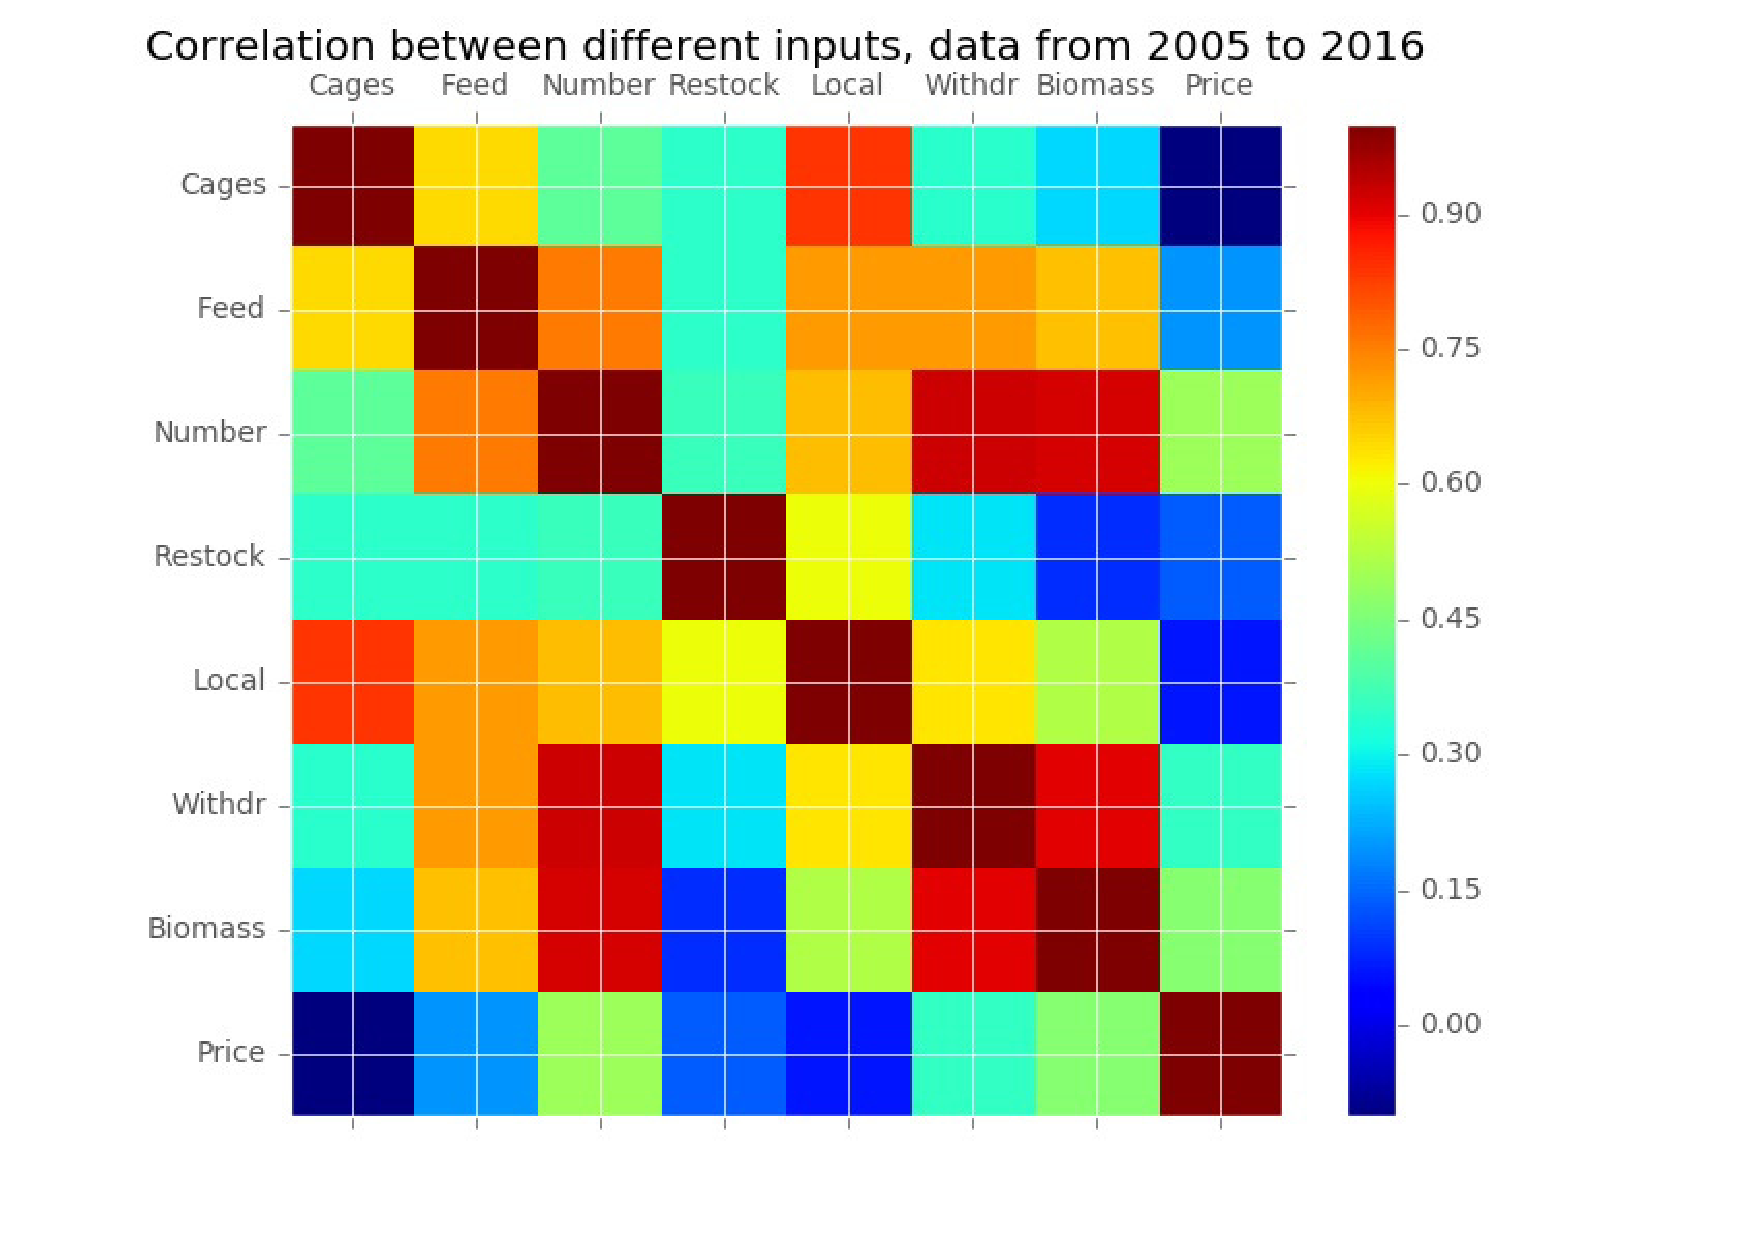
\includegraphics[width=0.90\textwidth]{Files/Total_Dataset_Years_Matrix.pdf}
    \caption{Correlation matrix between different inputs with data from 2005 to 2016.}
\end{figure}

\begin{table}[ht] 
\makebox[\textwidth][c] {
\resizebox{1.2\textwidth}{!}{\begin{tabular}{ | l | l | l | l | l | l | l | l | l |}
        \hline
INPUTS	& Cages 		& Feed 			& Number		& Restock 		& Local 		& Withdr 		& Biomass 		& Price 				\\ \hline
Cages	& 1				& 0.6448344		& 0.40797741	& 0.34410821	& 0.83884439	& 0.33936479	& 0.26930856 	& -0.10039588			\\ \hline
Feed	& 0.6448344		& 1				& 0.75881783	& 0.34641801	& 0.71978989	& 0.71813577	& 0.67744274 	& 0.1978647				\\ \hline
Number	& 0.40797741	& 0.75881783	& 1				& 0.360713		& 0.68022293	& 0.92284513	& 0.9154197		& 0.49510642			\\ \hline
Restock	& 0.34410821	& 0.34641801	& 0.3607131		& 1 			& 0.603927		& 0.28273088	& 0.08706515 	& 0.13621911			\\ \hline
Local	& 0.83884439	& 0.71978989	& 0.68022293	& 0.60392701	& 1				& 0.63415072	& 0.52016376 	& 0.0626106				\\ \hline
Withdr	& 0.33936479	& 0.71813577	& 0.92284513	& 0.28273088	& 0.63415072	& 1				& 0.90504847 	& 0.35208291			\\ \hline
Biomass	& 0.26930856	& 0.67744274	& 0.9154197		& 0.08706515	& 0.52016376	& 0.90504847	& 1 			& 0.46342121			\\ \hline
Price	& -0.10039588	& 0.1978647		& 0.49510642	& 0.13621911	& 0.0626106		& 0.35208291	& 0.46342121 	& 1						\\ \hline
    \end{tabular}}}
    \caption{Dataset inputs correlation coefficients value.}
    \label{table: trendline} 
\end{table}


\begin{figure}[H]
	\centering
    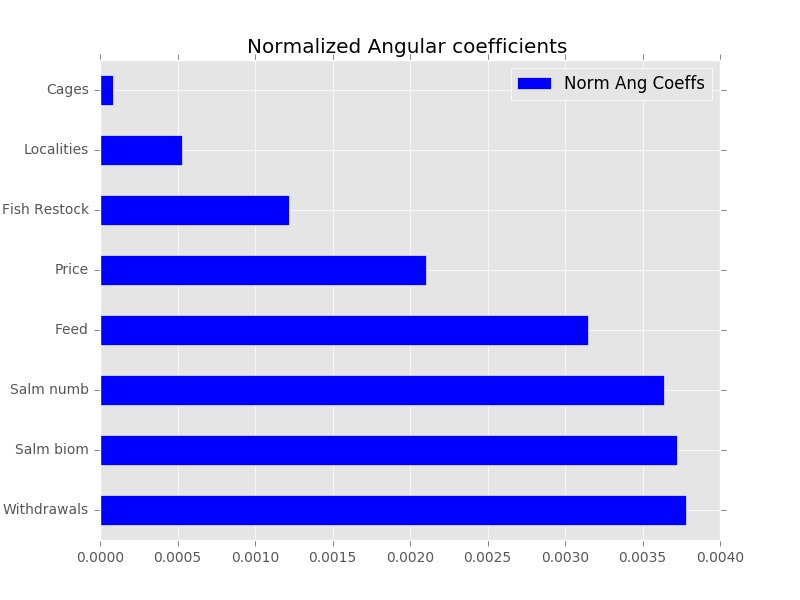
\includegraphics[width=0.75\textwidth]{Files/Norm_Ang_Coeffs.jpg}
    \caption{Normalized angular coefficients of each input's trendline.}
\end{figure}

\begin{table}[ht] 
	\centering
    \begin{tabular}{ | l | l | l | p{5cm} |}
        \hline
        Input 								& Equation 							& Coeff			\\ \hline
          	Salmon\_withdrawals 			& y=464.755139x+(46295.729945) 		& 464.755139 	\\ \hline
          	Salmon\_biomass\_end\_month 	& y=2832.712270x+(354138.727889) 	& 2832.71227 	\\ \hline
          	Salmon\_number\_end\_month 		& y=1543.298421x+(205325.455772)	& 1543.298421 	\\ \hline
          	Salmon\_consumption\_of\_feed 	& y=620.070855x+(58330.012273) 		& 620.070855	\\ \hline
           	Monthly\_salmon\_price 			& y=0.016952x+(4.293416) 			& 0.016952 		\\ \hline
          	Salmon\_restock 				& y=89.230600x+(13390.363406)		& 89.2306 		\\ \hline
 			Localities 						& y=0.343533x+(539.979023) 			& 0.343533		\\ \hline
  			Cages 							& y=0.342834x+(3665.904023) 		& 0.342834 		\\ \hline
    \end{tabular} 
    \caption{Dataset inputs trendline equation}
    \label{table: trendline} 
\end{table}
\begin{table}[ht] 
	\centering
    \begin{tabular}{ | l | l | l | p{5cm} |}
        \hline
        Input 							& Normalized equation 	& Norm Ang Coeffs	\\ \hline
          	Salmon\_withdrawals 		& y=0.003782x+(0.376694)& 0.003782			\\ \hline
          	Salmon\_biomass\_end\_month & y=0.003724x+(0.465599)& 0.003724			\\ \hline
          	Salmon\_number\_end\_month 	& y=0.003639x+(0.484184)& 0.003639			\\ \hline
          	Salmon\_consumption\_of\_feed & y=0.003147x+(0.296085)& 0.003147		\\ \hline
           	Monthly\_salmon\_price 		& y=0.002103x+(0.532682)& 0.002103			\\ \hline
          	Salmon\_restock 			& y=0.001217x+(0.182583)& 0.001217			\\ \hline
 			Localities 					& y=0.000531x+(0.834589)& 0.000531			\\ \hline
  			Cages 						& y=0.000082x+(0.877011)& 0.000082			\\ \hline
    \end{tabular} 
    \caption{Dataset inputs normalized trendline equation}
    \label{table: norm_trendline} 
\end{table}


\begin{figure}[H]
    \makebox[\textwidth][c]{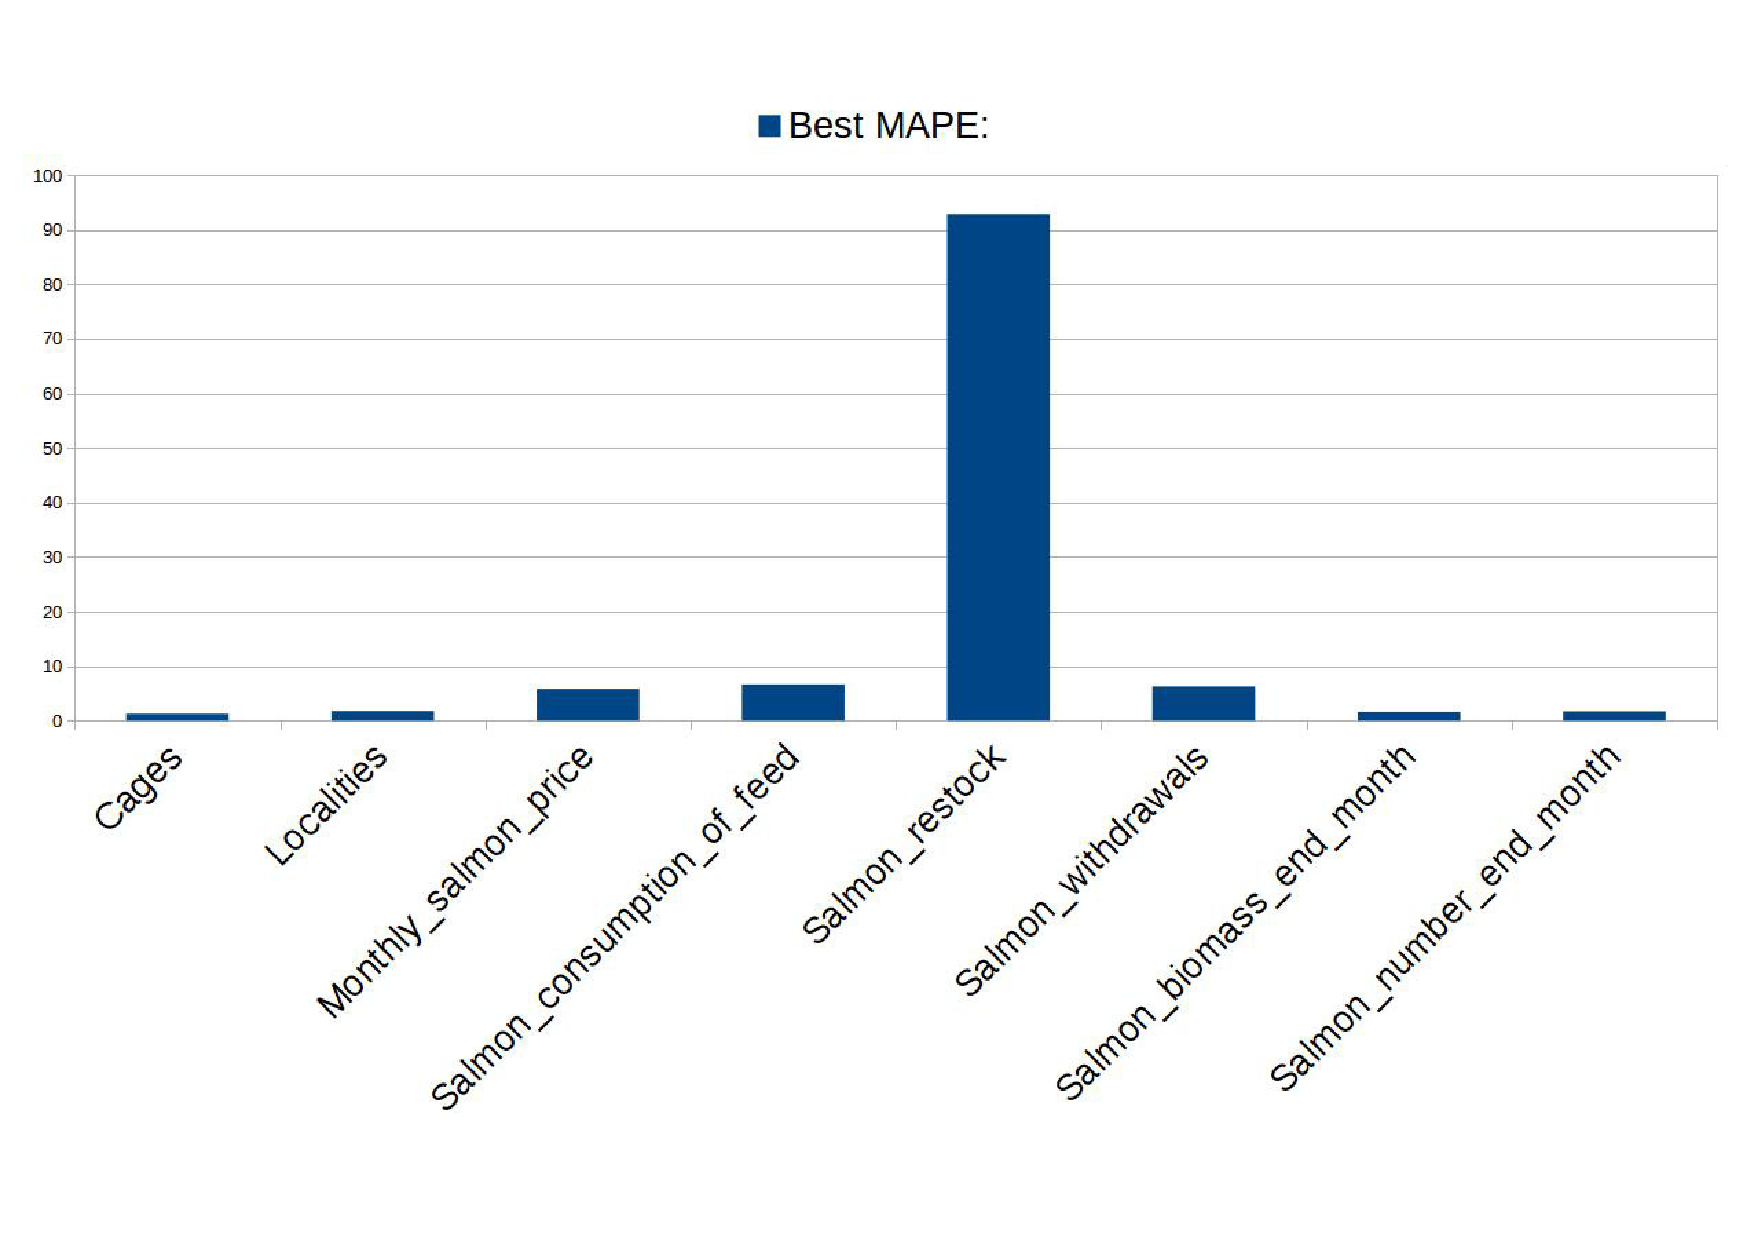
\includegraphics[width=1.2\textwidth]{Files/Best_MAPE.pdf}}
    \caption{Lower MAPE with best ARIMA Configuration for each tested input.}
\end{figure}

\begin{table}[ht] 
	\centering
    \begin{tabular}{ | l | l | l |}
            \hline
Input							&	ARIMA Conf	&	MAPE	\\ \hline
Cages							&	(10,2,1)	&	1.251\%	\\ \hline
Localities						&	(10,0,1)	&	1.779\%	\\ \hline
Monthly\_salmon\_price 			&	(2,0,0)		&	5.833\%	\\ \hline
Salmon\_consumption\_of\_feed	&	(6,1,0)		&	6.659\%	\\ \hline
Salmon\_restock 				&	(10,0,1)	&	96.006\%	\\ \hline
Salmon\_withdrawals 			&	(10,0,1)	&	6.277\%	\\ \hline
Salmon\_biomass\_end\_month		&	(8,1,0)		&	1.601\%	\\ \hline
Salmon\_number\_end\_month 		&	(10,2,0)	&	1.723\%	\\ \hline
    \end{tabular}  
    \caption{Dataset inputs normalized trendline equation}
    \label{table: Best ARIMA configurations with relative MAPE result in the Evaluation Test} 
\end{table}



\makebox[\textwidth][c]{
\resizebox{1.3\textwidth}{!}{
\begin{tabular}{|c|c|c|c|c|c|c|c|c|c|}
\hline
\multirow{3}{*}{Months} & \multicolumn{2}{c|}{Cages} & \multicolumn{2}{c|}{Localities} & \multicolumn{2}{c|}{Salmon Biomass} & \multicolumn{2}{c|}{Salmon Number}\\
\cline{2-9}
 & Real Values & Predictions & Real Values & Predictions & Real Values & Predictions & Real Values & Predictions \\
\hline
 January 2017 & 3436 & 3444.87 & & & & & &\\
\hline
 February 2017 & 3225 & 3251.915 & & & & & &\\
 \hline
 March 2017 & 3153 & 3164.190 & & & & & &\\
 \hline
 April 2017 & & 3317.814 & & & & & &\\
 \hline
 May 2017 & & 3492.701 & & & & & &\\
 \hline
 June 2017 & & 3507.062 & & & & & &\\
 \hline
 July 2017 & & 3485.804 & & & & & &\\
 \hline
 August 2017 & & & & & & & &\\
 \hline
 September 2017 & & & & & & & &\\
 \hline
 October 2017 & & & & & & & &\\
 \hline
 November 2017 & & & & & & & &\\
 \hline
 December 2017 & & & & & & & &\\
 \hline
% etc. ...
\end{tabular}  }}


\makebox[\textwidth][c]{
\resizebox{1.3\textwidth}{!}{
\begin{tabular}{|c|c|c|c|c|c|c|c|c|c|}
\hline
\multirow{3}{*}{Months} & \multicolumn{2}{c|}{Consumption of feed} & \multicolumn{2}{c|}{Salmon restock} & \multicolumn{2}{c|}{Salmon Withdrawals} & \multicolumn{2}{c|}{Salmon price}\\
\cline{2-9}
 & Real Values & Predictions & Real Values & Predictions & Real Values & Predictions & Real Values & Predictions \\
\hline
 January 2017 &  &  & & & & & &\\
\hline
 February 2017 & & & & & & & &\\
 \hline
 March 2017 & & & & & & & &\\
 \hline
 April 2017 & & & & & & & &\\
 \hline
 May 2017 & & & & & & & &\\
 \hline
 June 2017 & & & & & & & &\\
 \hline
 July 2017 & & & & & & & &\\
 \hline
 August 2017 & & & & & & & &\\
 \hline
 September 2017 & & & & & & & &\\
 \hline
 October 2017 & & & & & & & &\\
 \hline
 November 2017 & & & & & & & &\\
 \hline
 December 2017 & & & & & & & &\\
 \hline
% etc. ...
\end{tabular}  }}

\makebox[\textwidth][c]{
\resizebox{1.3\textwidth}{!}{
\begin{tabular}{|c|c|c|c|c|c|c|c|}

	\hline
     Input & Type & January 2017 & February 2017 & March 2017 & April 2017 & May 2017 & June 2017 \\ 
    \hline
    \multirow{2}{*}{Cages} &Real &3436 &3225 & & & &\\&Predicted &3444.87 &3251.915 & & & & \\
    \hline
    \multirow{2}{*}{Localities} &Real & & & & & &\\&Predicted & & & & & &\\
    \hline
    \multirow{2}{*}{Salmon Biomass} &Real & & & & & &\\&Predicted & & & & & &\\
    \hline
    \multirow{2}{*}{Salmon Number} &Real & & & & & &\\&Predicted & & & & & & \\
    \hline
   

\end{tabular}}}

